As described in Section.~\ref{sec:4.2}, JES and JER systematic uncertainties are considered for the String resonances. In this study, three NPs from the JES and 7 NPs from the JER are studied on the normalised template shapes. 

The impact from JES on the signal template is evaluated by comparing the nominal distribution to the distribution from each JES NP. The impact from JER on the signal template is estimated by examining the shift in the RMS (or standard deviation) of the distribution from each JER NP. Such signal shits are parameterised by fitting a Gaussian function to the most significant bins surrounding the maximum mean value of the distribution.


Figure~\ref{fig2} shows an example for the $\Ms = 8$~TeV signal sample.
This histogram exemplifies one of the systematic variations employed in the subsequent limit calculation. Among the various systematic sources, GroupedNP\_3 emerges as having the most substantial impact, leading to a significant shift in the signal mean.Across signal samples of diverse masses and widths, the reconstructed peak of the signal demonstrates a shift towards lower values in comparison to the generated peak, amounting to approximately $0.92 \times \Ms$. It is important to note that this shift is present even before accounting for the JES or JER systematic uncertainties.

\begin{figure}[htb]
\begin{center}
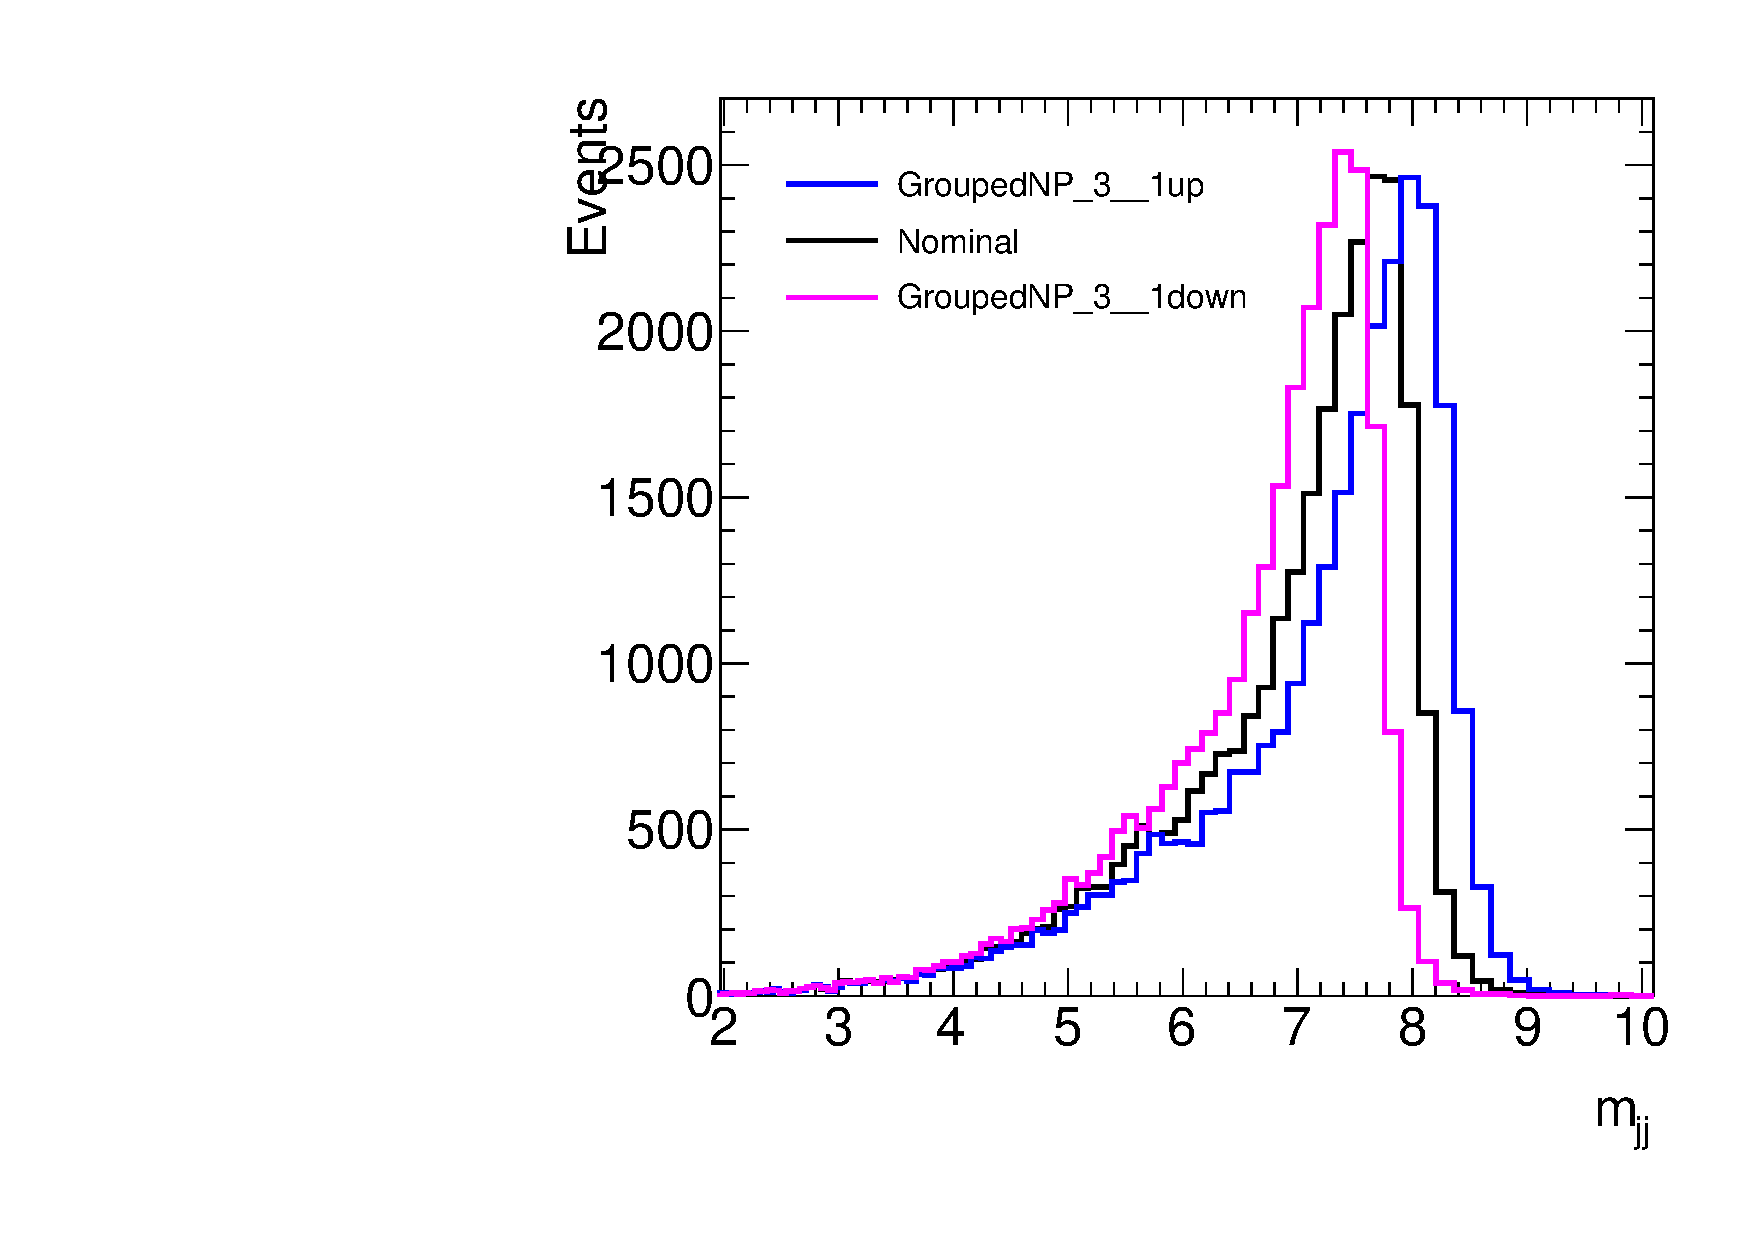
\includegraphics[width=0.65\linewidth]{fig/strings/JES_shift}
\end{center}
\caption{\mjj\ distribution for the $\Ms = 8$~TeV string sample (nominal).
Also shown are the distributions using the jet energy scale
GroupedNP\_3 one standard deviation up and down systematic uncertainties.}
\label{fig2}
\end{figure}

In Figure~\ref{fig3}, the proportional shift in the mean of the \mjj\ distribution attributed to the JES uncertainty and the relative change in RMS
of the \mjj\ distribution due to the JER uncertainty are depicted.
While all the NPs are independently incorporated in the limit computations, this illustration presents a combined display of the three JES mean shifts in quadrature and the seven JER resolution differences in quadrature.

\begin{figure}[htb]
\begin{center}
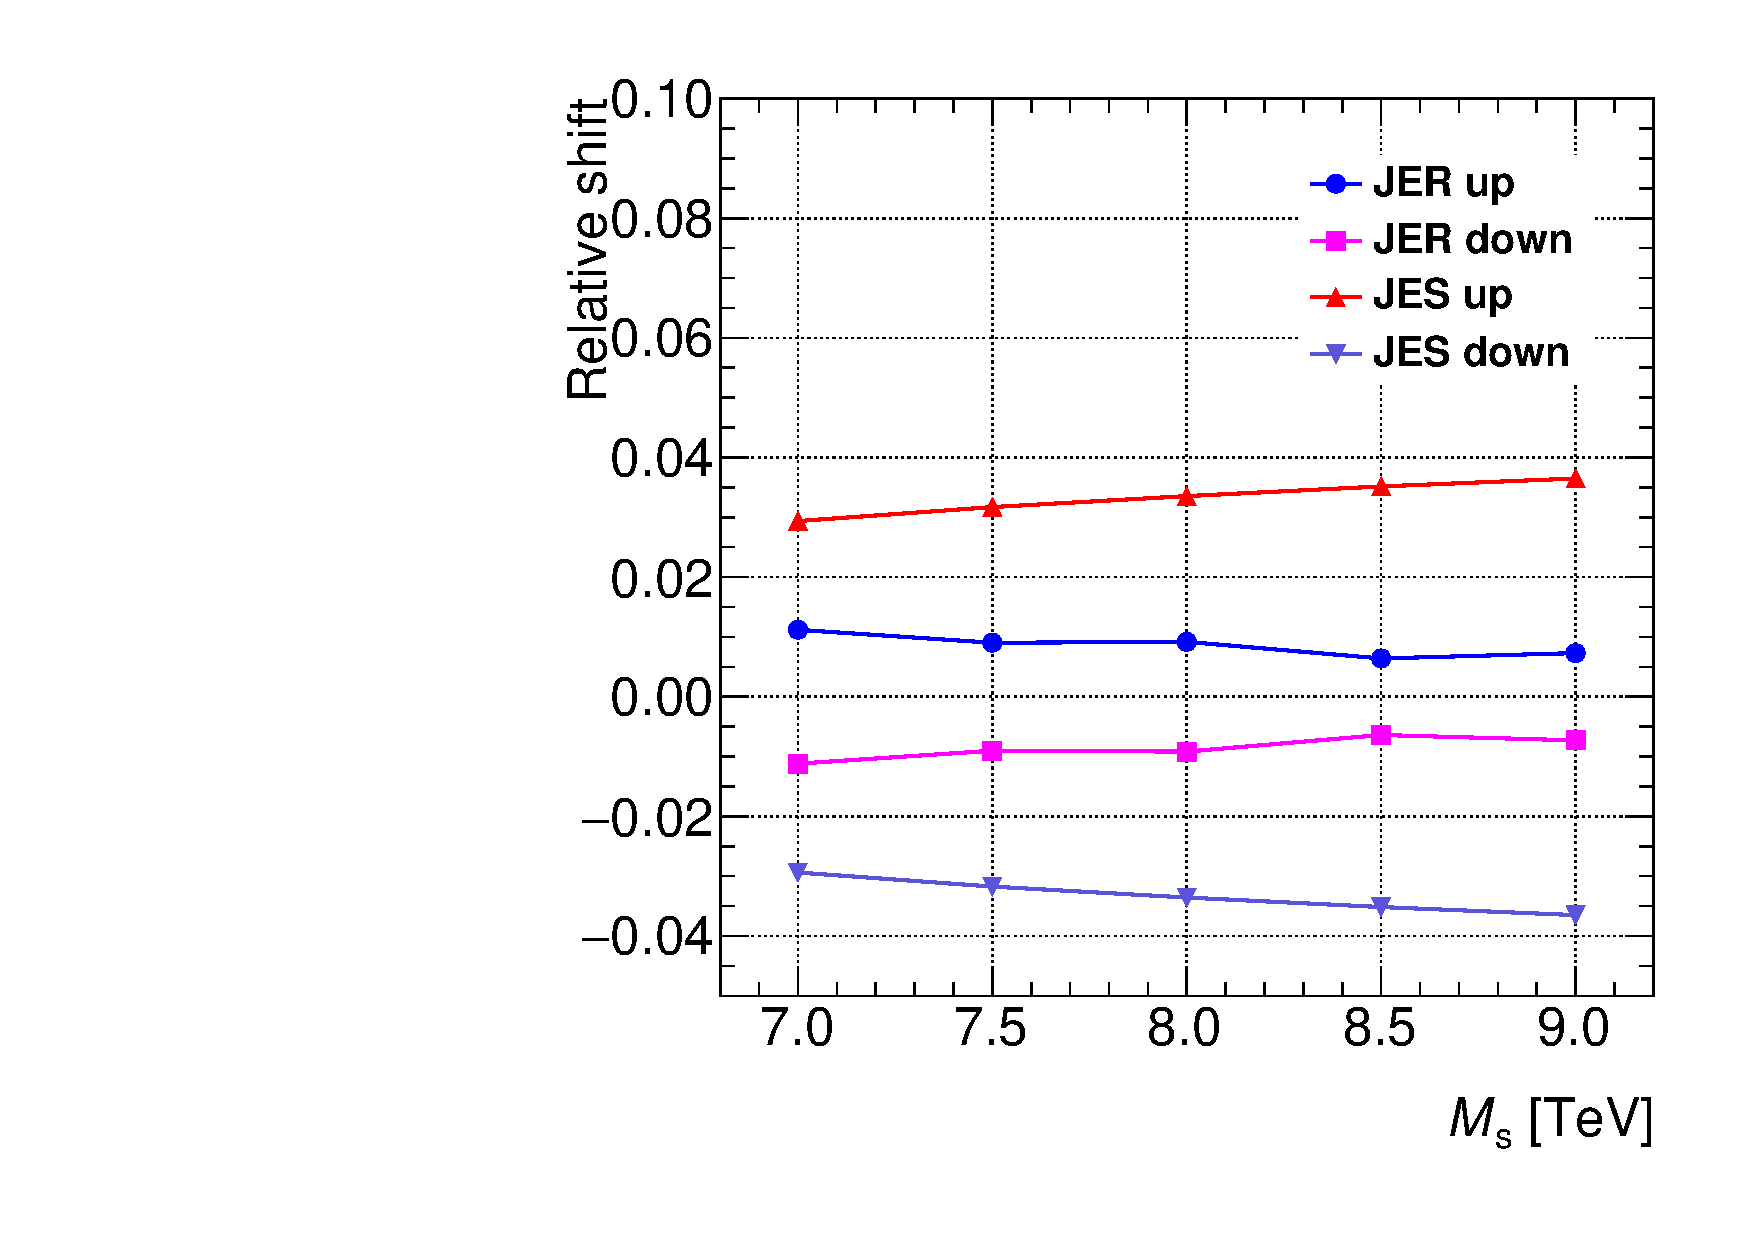
\includegraphics[width=0.65\linewidth]{fig/strings/JES_JER}
\end{center}
\caption{Relative shift in the mean of the \mjj\ distributions for each
string sample due to jet energy scale uncertainty, and relative change
in the RMS of the \mjj\ distributions for each string sample due to the
jet energy resolution uncertainty.
The changes due to each nuisance parameter group are added in
quadrature.}
\label{fig3}
\end{figure}

The alterations in signal acceptance from the inclusion of JES and JER uncertainties are
combined in quadrature and determined to be less than 0.06\%.  Such small uncertainty can be ignored for the signal
acceptance.


The shifts in the mean of the signal distributions, resulting from the inclusion of JES uncertainty, are primarily driven by GroupedNP\_3 and amount to less than 4\%.  Conversely, the alterations in the RMS of the signal distributions following the incorporation of JER uncertainty
remain below 1.2\%. Among the seven values combined in quadrature, none exhibit a dominant influence. Notably, the JER uncertainty emerges as the most substantial source of uncertainty for the lowest \Ms\ signal sample.


\FloatBarrier